\section{EXPERIMENT}\label{sec:exp}
The goal of throwing a projectile was set to 3.0m, the maximum usable distance in the SISTR system as described in Section~\ref{sec:intro}.  The target is placed directly in front of the robot.  Using the SRM the release point for the projectile motion calculations was set to the mean of the right arm's reachable area, 0.8m from the ground in $z$.  This resulted in a throwing velocity of 4.9m/s at $[\Theta, \Psi, \Phi] =[0.0^o,45.0^o, 3.8^o]$.  This velocity was required to be sustained for 0.1sec due to the speed and accuracy of the gripper's release.  This velocity duration and direction forced the trajectory to produce an underhand throwing gesture.  The projectile is a standard racquetball measuring 57mm in diameter and weighting 42.7g.  The light weight racquetball ball was chosen to assist in not causing instability.  $L_d$ and the setup trajectory are created using the method shown in Section~\ref{sec:methodology} and following all specified constraints.  Fig.~\ref{fig:sparseRegion} shows $L_d$ and the setup trajectory plotted within the SRM.

%\begin{figure}[thpb]
%  \centering
%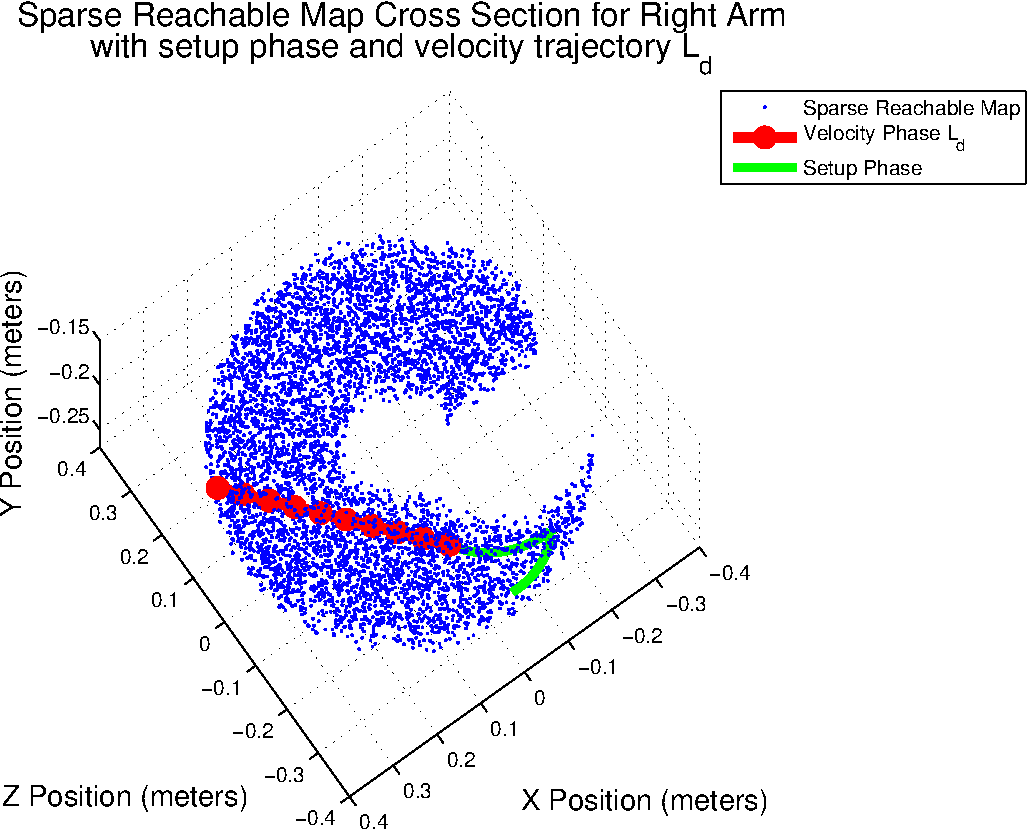
\includegraphics[width=1.0\columnwidth]{./MATLAB/throwTraj3D.pdf}
%  \caption{Sparse Reachable Map Cross Section for Right Arm with setup phase and velocity trajectory $L_d$ }
%  \label{fig:3dThrowPlot1}
%\end{figure}


\begin{figure}[thpb]
  \centering
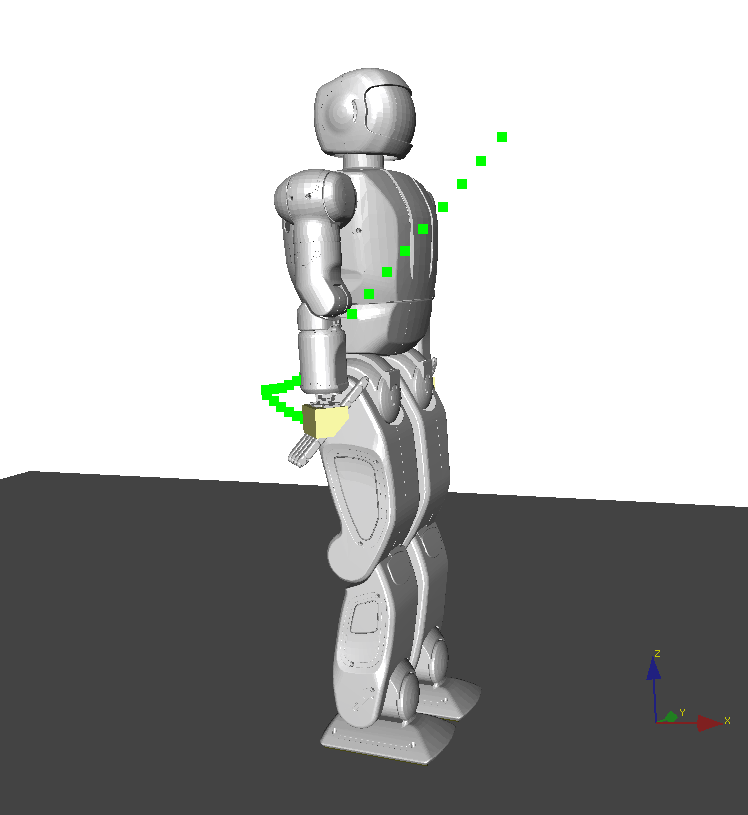
\includegraphics[width=0.25\columnwidth]{./pictures/ddFinal/vHside1.png}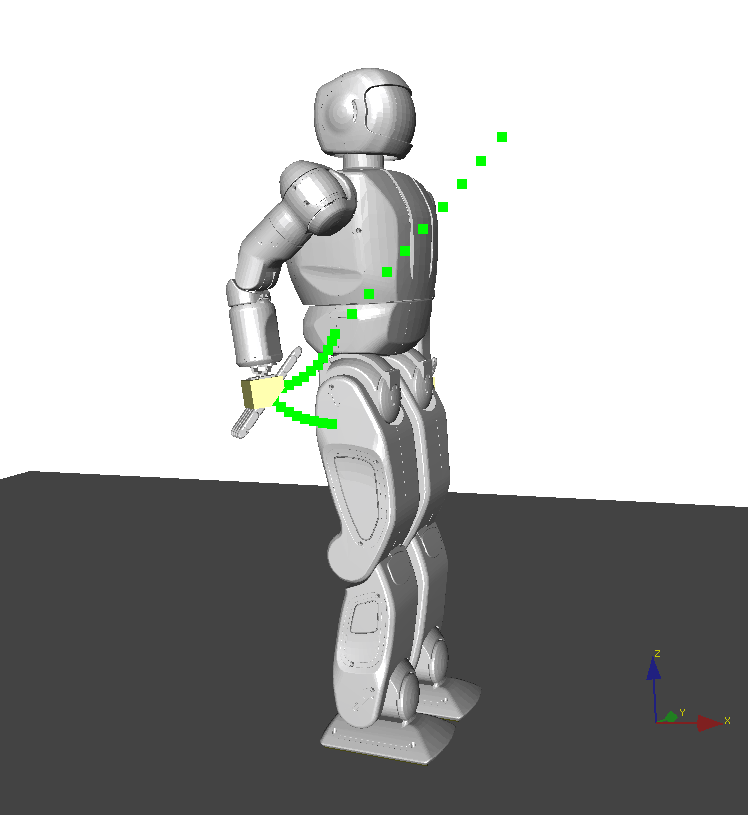
\includegraphics[width=0.25\columnwidth]{./pictures/ddFinal/vHside3.png}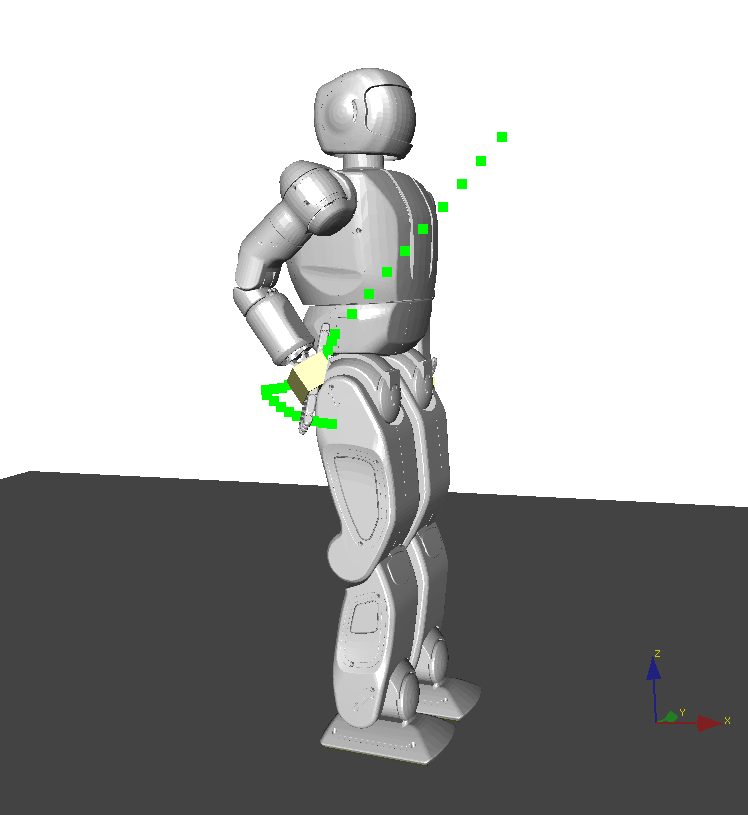
\includegraphics[width=0.25\columnwidth]{./pictures/ddFinal/vHside4.png}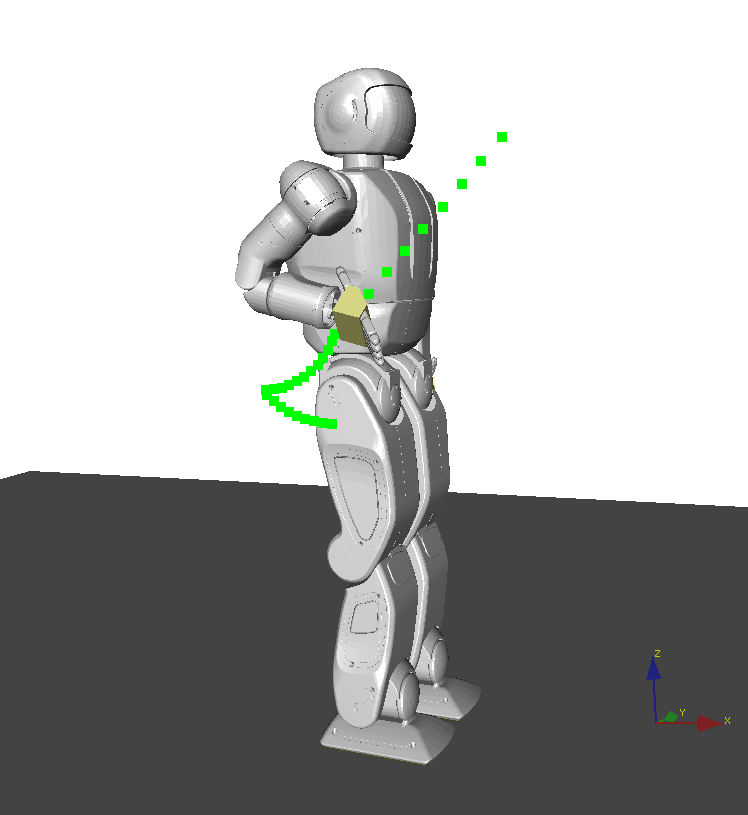
\includegraphics[width=0.25\columnwidth]{./pictures/ddFinal/vHside5.png}
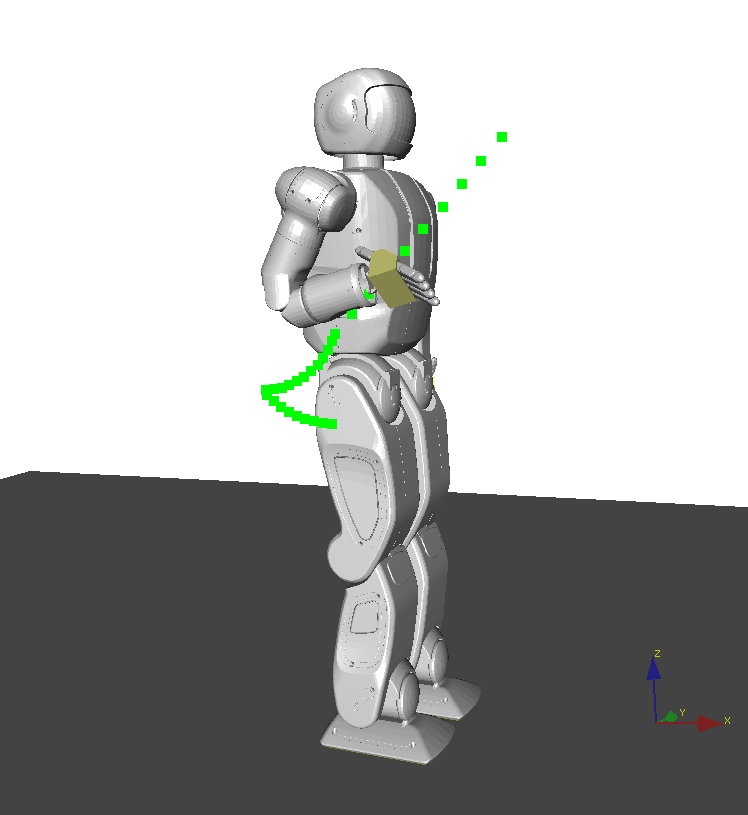
\includegraphics[width=0.25\columnwidth]{./pictures/ddFinal/vHside6.png}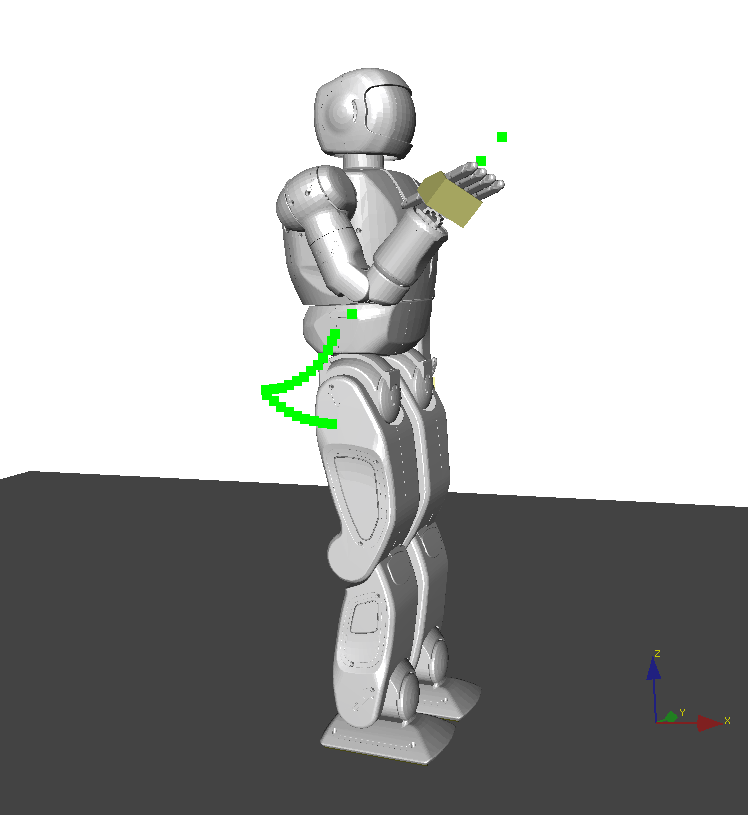
\includegraphics[width=0.25\columnwidth]{./pictures/ddFinal/vHside7.png}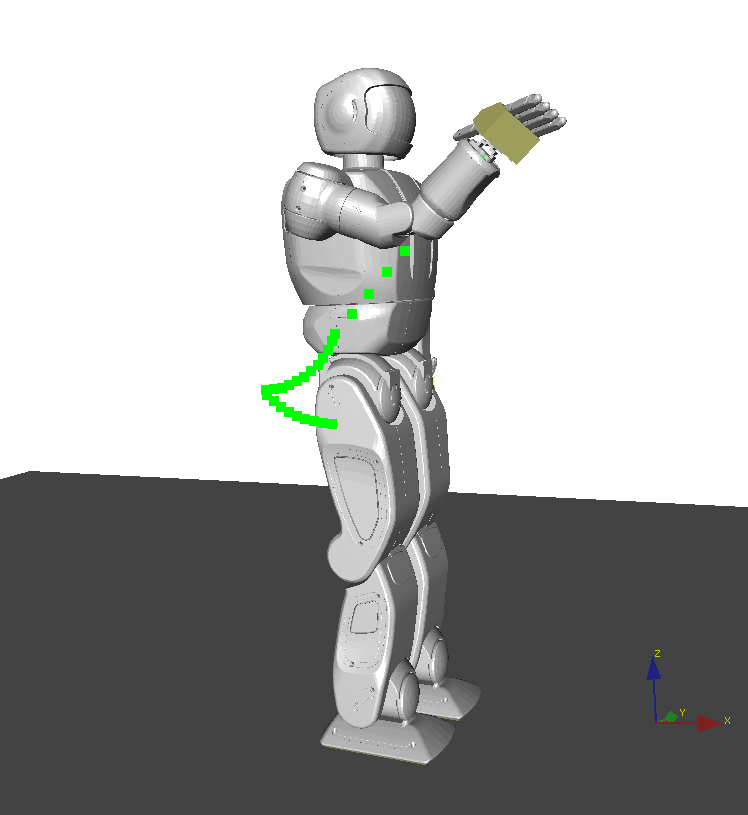
\includegraphics[width=0.25\columnwidth]{./pictures/ddFinal/vHside9.png}
  \caption{Jaemi Hubo running throwing trajectory $L_d$ immediately after the setup phase is completed.  $L_d(0)$ is top left.  Frames are read left to right and have a $\Delta t$ of 0.15s}
  \label{fig:fThrow}
\end{figure}



The trajectory was run on Jaemi Hubo with a position command period $T_r$ of 0.01s.  Fig~\ref{fig:3dThrowReal} shows the side profile of the Jaemi Hubo successfully running the trajectory.  The trajectory shown in Fig~\ref{fig:3dThrowReal} is considered an underhand throw, overhand and sidearm throws are also created with this method.

\begin{figure}[thpb]
  \centering
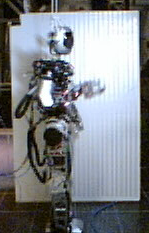
\includegraphics[width=0.25\columnwidth]{./pictures/slowMotion/1.png}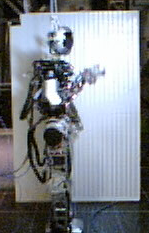
\includegraphics[width=0.25\columnwidth]{./pictures/slowMotion/2.png}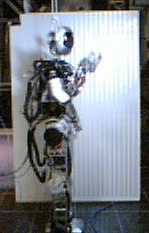
\includegraphics[width=0.25\columnwidth]{./pictures/slowMotion/3.png}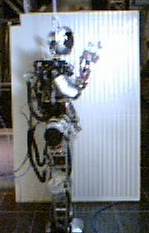
\includegraphics[width=0.25\columnwidth]{./pictures/slowMotion/4.png}
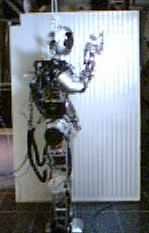
\includegraphics[width=0.25\columnwidth]{./pictures/slowMotion/5.png}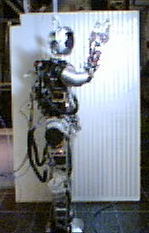
\includegraphics[width=0.25\columnwidth]{./pictures/slowMotion/6.png}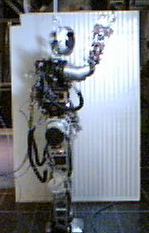
\includegraphics[width=0.25\columnwidth]{./pictures/slowMotion/7.png}
  \caption{Jaemi Hubo running throwing trajectory $L_d$ immediately after the setup phase is completed.  $L_d(0)$ is top left.  Frames are read left to right and have a $\Delta t$ of 0.15s}
  \label{fig:3dThrowReal}
\end{figure}

During the experiments the actual position of each joint was recorded.  The total time from the start of the setup phase to the end of the velocity phase is 0.31s.

